%=====================================================================
%==========================PAQUETES y DEFICION DEL ARCHIVO============
\documentclass[12pt]{article}
\usepackage[spanish,mexico]{babel}
	\selectlanguage{spanish}
\usepackage{graphicx}
\usepackage{amsmath}
\usepackage{wrapfig}
\usepackage{float}
\usepackage[utf8]{inputenc}
\usepackage[utf8]{inputenc}
\usepackage{color}
\usepackage{hyperref}
\usepackage{graphicx}
\graphicspath{{images/}}

\setlength{\parskip}{\medskipamount}
\setlength{\parindent}{0pt}
\definecolor{labelcolor}{RGB}{100,0,0}


\usepackage{vmargin}
\setmarginsrb{3 cm}{1.0 cm}{3 cm}{1.0 cm}{1 cm}{1.5 cm}{1 cm}{1.5 cm}
\usepackage{listings}
%=====================================================================
%=======================DATOS AUTOR===================================
%=====================================================================
\title{Actividad 8: Iniciandose en Computo Simbolico con Maxima}
\author{Martin Alejandro Paredes Sosa}
\date{Abril, 2016}
%=====================================================================
%=====================================================================
\begin{document}
\maketitle
%====================================================
%====================================================

\section{Introducción}
Maxima es una herramienta de de cálculo bastante versátil. Es un sistema para la manipulación de expresiones simbólicas y numéricas, incluyendo diferenciación, integración, ecuaciones diferenciales ordinarias, sistema de ecuaciones linales, vectores, matrices, entre otros. Maxima produce resultados de alta precisión. Adicionalmete permirte la graficación de funciones y datos en dos y tres dimensiones. \cite{M}

\begin{figure}[H]
\centering
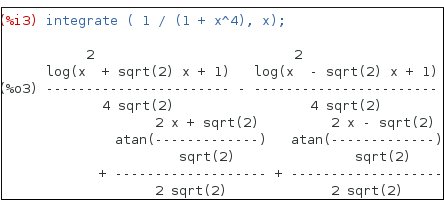
\includegraphics[scale=1]{maxi.png}
\caption{Interfaz de Maxima}
\end{figure}

\hspace{0.5cm} Para esta practica se nos pidió familiarizarnos con esta herramienta. Para esto se utilizó el manual de Jay Kerns sobre calculo de varias variables \cite{JK}, recreando los ejemplos que se mostraban. Para la realización de esta práctica, se utilzó wxMaxima, el cual es una interfaz grafica para trabajar con los comandos de Maxima.


\pagebreak

%====================================================
%====================================================

\section{Geometria en tres dimensiones}
Esta sección consta en enseñarnos herramientas para geometria tridimensional.
%====================================================
\subsection{Vectores y Algebra lineal}
En maxima hay forma de realizar operaciones con vectores, como es el producto punto y el producto cruz.

\noindent

\begin{minipage}[t]{8ex}{\color{red}\bf
\begin{verbatim}
(%i1) 
\end{verbatim}}
\end{minipage}
\begin{minipage}[t]{\textwidth}{\color{blue}
\begin{verbatim}
a: [6,2,5];
b: [8,-3,0];
a.b;
load(vect);
express(a~b);
c: [-5,2,9];
express(a.(b~c));
\end{verbatim}}
\end{minipage}

\begin{math}\displaystyle
\parbox{8ex}{\color{labelcolor}(\%o1) }
[6,2,5]
\end{math}

\begin{math}\displaystyle
\parbox{8ex}{\color{labelcolor}(\%o2) }
[8,-3,0]
\end{math}

\begin{math}\displaystyle
\parbox{8ex}{\color{labelcolor}(\%o3) }
42
\end{math}

\begin{math}\displaystyle
\parbox{8ex}{\color{labelcolor}(\%o4) }
/usr/share/maxima/5.34.1/share/vector/vect.mac
\end{math}

\begin{math}\displaystyle
\parbox{8ex}{\color{labelcolor}(\%o5) }
[15,40,-34]
\end{math}

\begin{math}\displaystyle
\parbox{8ex}{\color{labelcolor}(\%o6) }
[-5,2,9]
\end{math}

\begin{math}\displaystyle
\parbox{8ex}{\color{labelcolor}(\%o7) }
-301
\end{math}

%====================================================
%====================================================
\subsection{Lineas, Planos y Superficies Cuadraticas}
Con maxima se pueden definir ecuaciones de planos y superficies, con el objetivo de poder visualizarlos.

\begin{minipage}[t]{8ex}{\color{red}\bf
\begin{verbatim}
(%i1) 
\end{verbatim}}
\end{minipage}
\begin{minipage}[t]{\textwidth}{\color{blue}
\begin{verbatim}
load(draw);
ellips1: x^2/3+0.5*x*y+z   = 0;
draw3d(enhanced3d = true,
       palette = [cyan,blue,cyan],
       implicit(ellips1, x,-100,100, y,-100,100, z,-100,100));
\end{verbatim}}
\end{minipage}

\begin{math}\displaystyle
\parbox{8ex}{\color{labelcolor}(\%o1) }
/usr/share/maxima/5.34.1/share/draw/draw.lisp
\end{math}

\begin{math}\displaystyle
\parbox{8ex}{\color{labelcolor}(\%o2) }
z+0.5\,x\,y+\frac{{x}^{2}}{3}=0
\end{math}

\begin{math}\displaystyle
\parbox{8ex}{\color{labelcolor}(\%o3) }
[\mathrm{gr3d}\left( implicit\right) ]
\end{math}
\begin{figure}[H]
\centering
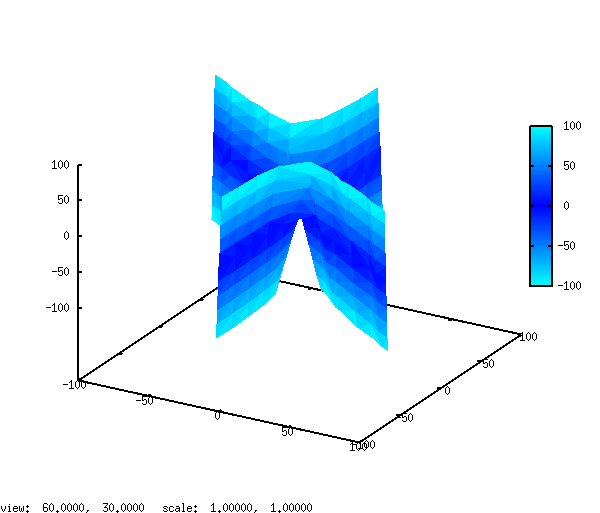
\includegraphics[scale=0.5]{1.png}
\caption{Grafica de la superficie $z+0.5\,x\,y+\frac{{x}^{2}}{3}=0$}
\end{figure}
%====================================================
%====================================================
\subsection{Funciones Vectoriales}
Maxima nos permite trabajar con funciones vectoriales como graficar, parametrizar y realizar operaciones con ellas.

\noindent
\begin{minipage}[t]{8ex}{\color{red}\bf
\begin{verbatim}
(%i1) 
\end{verbatim}}
\end{minipage}
\begin{minipage}[t]{\textwidth}{\color{blue}
\begin{verbatim}
load(draw);
load(eigen);
load(vect);
draw3d(parametric(cos(t),cos(4*t),-sin(t),t, -4,4));
r(t) := [cos(t), sin(t), t];
float(r(1));
limit(r(t),t,2);
limit(r(t),t, 2, plus);
limit(r(t), t,3,minus);
define(rp(t), diff(r(t),t));
float(rp(1));
define( T(t), trigsimp( uvect( rp(t) ) ) );
define(Tp(t), diff( T(t), t));
define( N(t), trigsimp( uvect( Tp(t) ) ) );
express(T(t)~N(t));
define(B(t),trigsimp(%));
float(B(1));
\end{verbatim}}
\end{minipage}
%%% OUTPUT:
\begin{math}\displaystyle
\parbox{8ex}{\color{labelcolor}(\%o1) }
/usr/share/maxima/5.34.1/share/draw/draw.lisp
\end{math}

\begin{math}\displaystyle
\parbox{8ex}{\color{labelcolor}(\%o2) }
/usr/share/maxima/5.34.1/share/matrix/eigen.mac
\end{math}

\begin{math}\displaystyle
\parbox{8ex}{\color{labelcolor}(\%o3) }
/usr/share/maxima/5.34.1/share/vector/vect.mac
\end{math}

\begin{math}\displaystyle
\parbox{8ex}{\color{labelcolor}(\%o4) }
[\mathrm{gr3d}\left( parametric\right) ]
\end{math}

\begin{figure}[H]
\centering
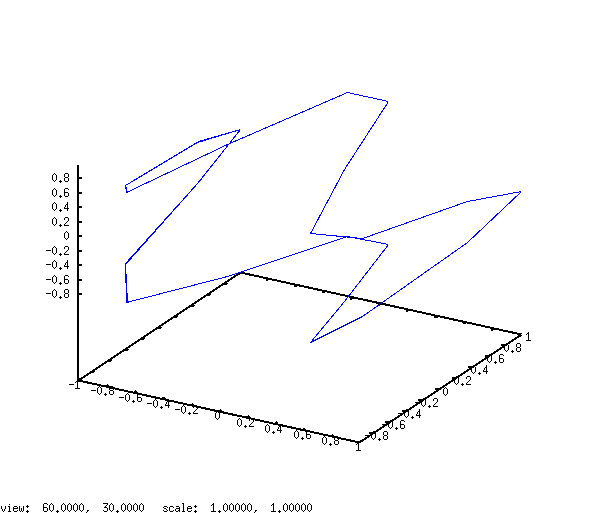
\includegraphics[scale=0.5]{2.png}
\caption{Trayectoria descrita por $(cos(t),cos(4*t),-sin(t))$ donde $t\in[-4,4]$ }
\end{figure}

\begin{math}\displaystyle
\parbox{8ex}{\color{labelcolor}(\%o5) }
\mathrm{r}\left( t\right) :=[\mathrm{cos}\left( t\right) ,\mathrm{sin}\left( t\right) ,t]
\end{math}

\begin{math}\displaystyle
\parbox{8ex}{\color{labelcolor}(\%o6) }
[0.5403023058681398,0.8414709848078965,1.0]
\end{math}

\begin{math}\displaystyle
\parbox{8ex}{\color{labelcolor}(\%o7) }
[\mathrm{cos}\left( 2\right) ,\mathrm{sin}\left( 2\right) ,2]
\end{math}

\begin{math}\displaystyle
\parbox{8ex}{\color{labelcolor}(\%o8) }
[\mathrm{cos}\left( 2\right) ,\mathrm{sin}\left( 2\right) ,2]
\end{math}

\begin{math}\displaystyle
\parbox{8ex}{\color{labelcolor}(\%o9) }
[\mathrm{cos}\left( 3\right) ,\mathrm{sin}\left( 3\right) ,3]
\end{math}

\begin{math}\displaystyle
\parbox{8ex}{\color{labelcolor}(\%o10) }
\mathrm{rp}\left( t\right) :=[-\mathrm{sin}\left( t\right) ,\mathrm{cos}\left( t\right) ,1]
\end{math}

\begin{math}\displaystyle
\parbox{8ex}{\color{labelcolor}(\%o11) }
[-0.8414709848078965,0.5403023058681398,1.0]
\end{math}

\begin{math}\displaystyle
\parbox{8ex}{\color{labelcolor}(\%o12) }
\mathrm{T}\left( t\right) :=[-\frac{\mathrm{sin}\left( t\right) }{\sqrt{2}},\frac{\mathrm{cos}\left( t\right) }{\sqrt{2}},\frac{1}{\sqrt{2}}]
\end{math}

\begin{math}\displaystyle
\parbox{8ex}{\color{labelcolor}(\%o13) }
\mathrm{Tp}\left( t\right) :=[-\frac{\mathrm{cos}\left( t\right) }{\sqrt{2}},-\frac{\mathrm{sin}\left( t\right) }{\sqrt{2}},0]
\end{math}

\begin{math}\displaystyle
\parbox{8ex}{\color{labelcolor}(\%o14) }
\mathrm{N}\left( t\right) :=[-\mathrm{cos}\left( t\right) ,-\mathrm{sin}\left( t\right) ,0]
\end{math}

\begin{math}\displaystyle
\parbox{8ex}{\color{labelcolor}(\%o15) }
[\frac{\mathrm{sin}\left( t\right) }{\sqrt{2}},-\frac{\mathrm{cos}\left( t\right) }{\sqrt{2}},\frac{{\mathrm{sin}\left( t\right) }^{2}}{\sqrt{2}}+\frac{{\mathrm{cos}\left( t\right) }^{2}}{\sqrt{2}}]
\end{math}

\begin{math}\displaystyle
\parbox{8ex}{\color{labelcolor}(\%o16) }
\mathrm{B}\left( t\right) :=[\frac{\mathrm{sin}\left( t\right) }{\sqrt{2}},-\frac{\mathrm{cos}\left( t\right) }{\sqrt{2}},\frac{1}{\sqrt{2}}]
\end{math}

\begin{math}\displaystyle
\parbox{8ex}{\color{labelcolor}(\%o17) }
[0.5950098395293859,-0.3820514243700897,0.7071067811865475]
\end{math}


\subsection{Longitud de Arco y Curvatura}
En maxima nos permite realizar las operaciones para calcular estas cualidades de ecuaciones paramétricas.

\noindent

\begin{minipage}[t]{8ex}{\color{red}\bf
\begin{verbatim}
(%i1) 
\end{verbatim}}
\end{minipage}
\begin{minipage}[t]{\textwidth}{\color{blue}
\begin{verbatim}
r(t) := [t, cos(t), sin(t)];
rp(t) := [1,-sin(t), cos(t)];
Tp(t) := [0,-cos(t), sin(t)]/sqrt(2);
sqrt(Tp(t) . Tp(t))/sqrt(rp(t).rp(t));
trigsimp(%);
define(kappa(t),%);
integrate(r(t),t);
g(t) := [2*t,3*sin(t),3*cos(t)];
define(gp(t) , diff(g(t),t));
integrate(trigsimp(sqrt(gp(t).gp(t))),t,0,2*%pi);
romberg(sqrt(gp(t).gp(t)),t,0,2*%pi);
\end{verbatim}}
\end{minipage}
%%% OUTPUT:
\begin{math}\displaystyle
\parbox{8ex}{\color{labelcolor}(\%o1) }
\mathrm{r}\left( t\right) :=[t,\mathrm{cos}\left( t\right) ,\mathrm{sin}\left( t\right) ]
\end{math}

\begin{math}\displaystyle
\parbox{8ex}{\color{labelcolor}(\%o2) }
\mathrm{rp}\left( t\right) :=[1,-\mathrm{sin}\left( t\right) ,\mathrm{cos}\left( t\right) ]
\end{math}

\begin{math}\displaystyle
\parbox{8ex}{\color{labelcolor}(\%o3) }
\mathrm{Tp}\left( t\right) :=\frac{[0,-\mathrm{cos}\left( t\right) ,\mathrm{sin}\left( t\right) ]}{\sqrt{2}}
\end{math}

\begin{math}\displaystyle
\parbox{8ex}{\color{labelcolor}(\%o4) }
\frac{\sqrt{\frac{{\mathrm{sin}\left( t\right) }^{2}}{2}+\frac{{\mathrm{cos}\left( t\right) }^{2}}{2}}}{\sqrt{{\mathrm{sin}\left( t\right) }^{2}+{\mathrm{cos}\left( t\right) }^{2}+1}}
\end{math}

\begin{math}\displaystyle
\parbox{8ex}{\color{labelcolor}(\%o5) }
\frac{1}{2}
\end{math}

\begin{math}\displaystyle
\parbox{8ex}{\color{labelcolor}(\%o6) }
\kappa\left( t\right) :=\frac{1}{2}
\end{math}

\begin{math}\displaystyle
\parbox{8ex}{\color{labelcolor}(\%o7) }
[\frac{{t}^{2}}{2},\mathrm{sin}\left( t\right) ,-\mathrm{cos}\left( t\right) ]
\end{math}

\begin{math}\displaystyle
\parbox{8ex}{\color{labelcolor}(\%o8) }
\mathrm{g}\left( t\right) :=[2\,t,3\,\mathrm{sin}\left( t\right) ,3\,\mathrm{cos}\left( t\right) ]
\end{math}

\begin{math}\displaystyle
\parbox{8ex}{\color{labelcolor}(\%o9) }
\mathrm{gp}\left( t\right) :=[2,3\,\mathrm{cos}\left( t\right) ,-3\,\mathrm{sin}\left( t\right) ]
\end{math}

\begin{math}\displaystyle
\parbox{8ex}{\color{labelcolor}(\%o10) }
2\,\sqrt{13}\,\pi 
\end{math}

\begin{math}\displaystyle
\parbox{8ex}{\color{labelcolor}(\%o11) }
22.65434679827795
\end{math}
%===================================================================
%===================================================================
\section{Funciones de varias varibles}
Maxima tiene la habilidad de trabajar con funciones de varias varibles, así como graficarlas.
\noindent
\begin{minipage}[t]{8ex}{\color{red}\bf
\begin{verbatim}
(%i1) 
\end{verbatim}}
\end{minipage}
\begin{minipage}[t]{\textwidth}{\color{blue}
\begin{verbatim}
load(draw);
f(x,y) := (5*x^2-2*y^2)^0.25;
draw3d(explicit(f(x,y),x,-5,5,y,-5,5));
\end{verbatim}}
\end{minipage}

\begin{math}\displaystyle
\parbox{8ex}{\color{labelcolor}(\%o1) }
/usr/share/maxima/5.34.1/share/draw/draw.lisp
\end{math}

\begin{math}\displaystyle
\parbox{8ex}{\color{labelcolor}(\%o2) }
\mathrm{f}\left( x,y\right) :={\left( 5\,{x}^{2}-2\,{y}^{2}\right) }^{0.25}
\end{math}

\begin{math}\displaystyle
\parbox{8ex}{\color{labelcolor}(\%o3) }
[\mathrm{gr3d}\left( explicit\right) ]
\end{math}

\begin{figure}[H]
\centering
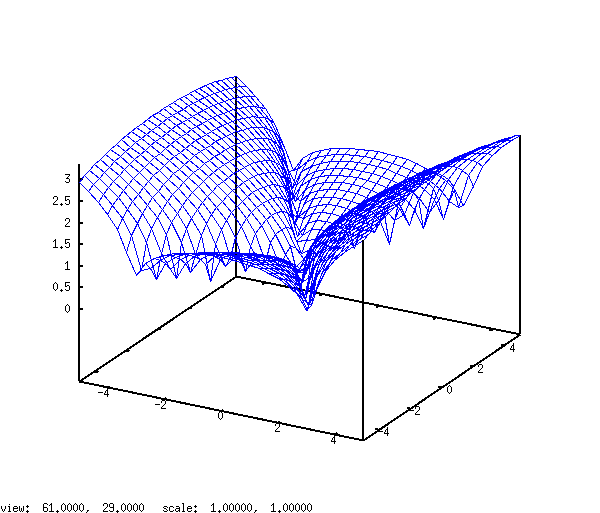
\includegraphics[scale=0.5]{3.png}
\caption{Superficie $f(x,y)= (5*x^2-2*y^2)^0.25$ }
\end{figure}

\noindent

\begin{minipage}[t]{8ex}{\color{red}\bf
\begin{verbatim}
(%i4) 
\end{verbatim}}
\end{minipage}
\begin{minipage}[t]{\textwidth}{\color{blue}
\begin{verbatim}
draw3d(enhanced3d = true,
       explicit(f(x,y),x,-5,5,y,-5,5),
       palette = [green,blue,cyan,red]);
\end{verbatim}}
\end{minipage}
:
\begin{math}\displaystyle
\parbox{8ex}{\color{labelcolor}(\%o4) }
[\mathrm{gr3d}\left( explicit\right) ]
\end{math}

\begin{figure}[H]
\centering
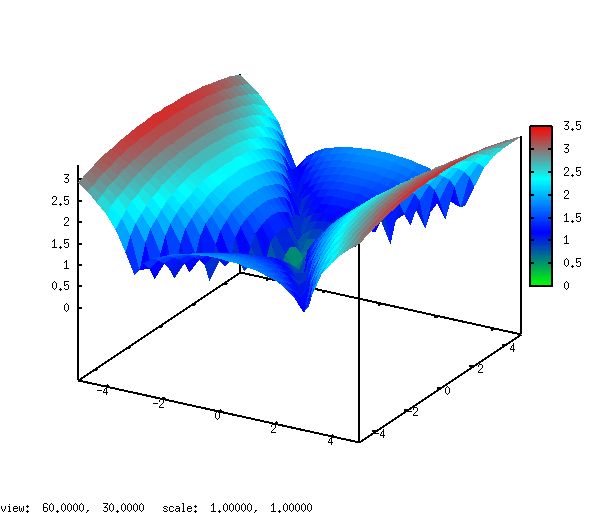
\includegraphics[scale=0.5]{4.png}
\caption{Superficie $f(x,y)= (5*x^2-2*y^2)^0.25$ }
\end{figure}

\noindent

\begin{minipage}[t]{8ex}{\color{red}\bf
\begin{verbatim}
(%i5) 
\end{verbatim}}
\end{minipage}
\begin{minipage}[t]{\textwidth}{\color{blue}
\begin{verbatim}
draw3d(explicit(f(x,y),x,-5,5,y,-5,5),
    contour_levels = 20,
    contour        = map);
\end{verbatim}}
\end{minipage}

\begin{math}\displaystyle
\parbox{8ex}{\color{labelcolor}(\%o5) }
[\mathrm{gr3d}\left( explicit\right) ]
\end{math}

\begin{figure}[H]
\centering
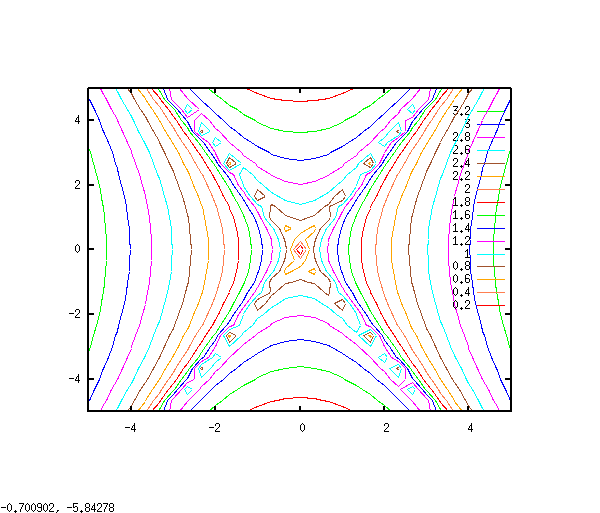
\includegraphics[scale=0.5]{5.png}
\caption{curvas de nivel de $f(x,y)= (5*x^2-2*y^2)^0.25$ }
\end{figure}

\noindent
\begin{minipage}[t]{8ex}{\color{red}\bf
\begin{verbatim}
(%i6) 
\end{verbatim}}
\end{minipage}
\begin{minipage}[t]{\textwidth}{\color{blue}
\begin{verbatim}
draw3d(enhanced3d = true,
       explicit(f(x,y),x,-5,5,y,-5,5),
       contour_levels = 20,
       contour = surface,
       palette = [green,blue,cyan,red],
       surface_hide = true);
\end{verbatim}}
\end{minipage}

\begin{math}\displaystyle
\parbox{8ex}{\color{labelcolor}(\%o6) }
[\mathrm{gr3d}\left( explicit\right) ]
\end{math}
\begin{figure}[H]
\centering
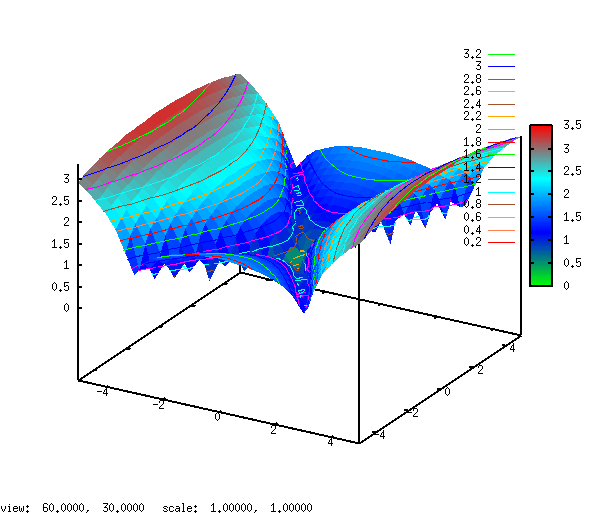
\includegraphics[scale=0.5]{6.png}
\caption{Superficie $f(x,y)= (5*x^2-2*y^2)^0.25$ }
\end{figure}

%===============================================================

\subsection{Derivadas Parciales}
Maxima nos permite realizar derivadas parciales 
\noindent

\begin{minipage}[t]{8ex}{\color{red}\bf
\begin{verbatim}
(%i1) 
\end{verbatim}}
\end{minipage}
\begin{minipage}[t]{\textwidth}{\color{blue}
\begin{verbatim}
diff(f(x,y),x,2,y,1,x,2);
G : (1/32)*x^7*y^8;
diff(G , x,2, y,1 , x,2);
\end{verbatim}}
\end{minipage}

\begin{math}\displaystyle
\parbox{8ex}{\color{labelcolor}(\%o1) }
\frac{{d}^{5}}{d\,{x}^{4}\,d\,y}\,\mathrm{f}\left( x,y\right) 
\end{math}

\begin{math}\displaystyle
\parbox{8ex}{\color{labelcolor}(\%o2) }
\frac{{x}^{7}\,{y}^{8}}{32}
\end{math}

\begin{math}\displaystyle
\parbox{8ex}{\color{labelcolor}(\%o3) }
210\,{x}^{3}\,{y}^{7}
\end{math}

%====================================================

\subsection{Aproximación Lineal y Diferenciales}
Con Maxima podemos realizar aproximaciones de funciones y ademas de poder expresar los diferenciales de las expresiones.
\noindent

\begin{minipage}[t]{8ex}{\color{red}\bf
\begin{verbatim}
(%i1) 
\end{verbatim}}
\end{minipage}
\begin{minipage}[t]{\textwidth}{\color{blue}
\begin{verbatim}
f(x,y) := exp(x) * cos(y^2);
\end{verbatim}}
\end{minipage}

\begin{math}\displaystyle
\parbox{8ex}{\color{labelcolor}(\%o1) }
\mathrm{f}\left( x,y\right) :=\mathrm{exp}\left( x\right) \,\mathrm{cos}\left( {y}^{2}\right) 
\end{math}


\noindent

\begin{minipage}[t]{8ex}{\color{red}\bf
\begin{verbatim}
(%i2) 
\end{verbatim}}
\end{minipage}
\begin{minipage}[t]{\textwidth}{\color{blue}
\begin{verbatim}
taylor(f(x,y), [x,y],[1,2],1);
\end{verbatim}}
\end{minipage}

\begin{math}\displaystyle
\parbox{8ex}{\color{labelcolor}(\%o2)/T/ }
\mathrm{cos}\left( 4\right) \,e+\left( \mathrm{cos}\left( 4\right) \,e\,\left( x-1\right) -4\,\mathrm{sin}\left( 4\right) \,e\,\left( y-2\right) \right) +...
\end{math}


\noindent

\begin{minipage}[t]{8ex}{\color{red}\bf
\begin{verbatim}
(%i3) 
\end{verbatim}}
\end{minipage}
\begin{minipage}[t]{\textwidth}{\color{blue}
\begin{verbatim}
diff(f(x,y));
\end{verbatim}}
\end{minipage}

\begin{math}\displaystyle
\parbox{8ex}{\color{labelcolor}(\%o3) }
{e}^{x}\,\mathrm{cos}\left( {y}^{2}\right) \,\mathrm{del}\left( x\right) -2\,{e}^{x}\,y\,\mathrm{sin}\left( {y}^{2}\right) \,\mathrm{del}\left( y\right) 
\end{math}

%===========================================================

\subsection{Regla de la cadena y derivación implicita}
Se puede realizar la regla de la cadena y derivación implicita.
\noindent

\begin{minipage}[t]{8ex}{\color{red}\bf
\begin{verbatim}
(%i1) 
\end{verbatim}}
\end{minipage}
\begin{minipage}[t]{\textwidth}{\color{blue}
\begin{verbatim}
f(x,y):= exp(x^3)*sin(4*y);
[x,y] : [s^2*t, s*t^2];
\end{verbatim}}
\end{minipage}

\begin{math}\displaystyle
\parbox{8ex}{\color{labelcolor}(\%o1) }
\mathrm{f}\left( x,y\right) :=\mathrm{exp}\left( {x}^{3}\right) \,\mathrm{sin}\left( 4\,y\right) 
\end{math}

\begin{math}\displaystyle
\parbox{8ex}{\color{labelcolor}(\%o2) }
[{s}^{2}\,t,s\,{t}^{2}]
\end{math}

\noindent

\begin{minipage}[t]{8ex}{\color{red}\bf
\begin{verbatim}
(%i3) 
\end{verbatim}}
\end{minipage}
\begin{minipage}[t]{\textwidth}{\color{blue}
\begin{verbatim}
diff(f(x,y),s);
diff(f(x,y),t);
\end{verbatim}}
\end{minipage}

\begin{math}\displaystyle
\parbox{8ex}{\color{labelcolor}(\%o3) }
6\,{s}^{5}\,{t}^{3}\,{e}^{{s}^{6}\,{t}^{3}}\,\mathrm{sin}\left( 4\,s\,{t}^{2}\right) +4\,{t}^{2}\,{e}^{{s}^{6}\,{t}^{3}}\,\mathrm{cos}\left( 4\,s\,{t}^{2}\right) 
\end{math}

\begin{math}\displaystyle
\parbox{8ex}{\color{labelcolor}(\%o4) }
3\,{s}^{6}\,{t}^{2}\,{e}^{{s}^{6}\,{t}^{3}}\,\mathrm{sin}\left( 4\,s\,{t}^{2}\right) +8\,s\,t\,{e}^{{s}^{6}\,{t}^{3}}\,\mathrm{cos}\left( 4\,s\,{t}^{2}\right) 
\end{math}

\noindent

\begin{minipage}[t]{8ex}{\color{red}\bf
\begin{verbatim}
(%i5) 
\end{verbatim}}
\end{minipage}
\begin{minipage}[t]{\textwidth}{\color{blue}
\begin{verbatim}
diff(f(u,v),u);
kill(x,y);
diff(f(x,y),x);
\end{verbatim}}
\end{minipage}

\begin{math}\displaystyle
\parbox{8ex}{\color{labelcolor}(\%o5) }
3\,{u}^{2}\,{e}^{{u}^{3}}\,\mathrm{sin}\left( 4\,v\right) 
\end{math}

\begin{math}\displaystyle
\parbox{8ex}{\color{labelcolor}(\%o6) }
done
\end{math}

\begin{math}\displaystyle
\parbox{8ex}{\color{labelcolor}(\%o7) }
3\,{x}^{2}\,{e}^{{x}^{3}}\,\mathrm{sin}\left( 4\,y\right) 
\end{math}

\noindent

\begin{minipage}[t]{8ex}{\color{red}\bf
\begin{verbatim}
(%i8) 
\end{verbatim}}
\end{minipage}
\begin{minipage}[t]{\textwidth}{\color{blue}
\begin{verbatim}
F: 3*x*y^4*z^2 + 2*x*y*2*z-3*x*z-x;
Fx: diff(F,x);
Fy: diff(F,y);
Fz: diff(F,z);
[-Fx/Fy,-Fy/Fz];
\end{verbatim}}
\end{minipage}

\begin{math}\displaystyle
\parbox{8ex}{\color{labelcolor}(\%o8) }
3\,x\,{y}^{4}\,{z}^{2}+4\,x\,y\,z-3\,x\,z-x
\end{math}

\begin{math}\displaystyle
\parbox{8ex}{\color{labelcolor}(\%o9) }
3\,{y}^{4}\,{z}^{2}+4\,y\,z-3\,z-1
\end{math}

\begin{math}\displaystyle
\parbox{8ex}{\color{labelcolor}(\%o10) }
12\,x\,{y}^{3}\,{z}^{2}+4\,x\,z
\end{math}

\begin{math}\displaystyle
\parbox{8ex}{\color{labelcolor}(\%o11) }
6\,x\,{y}^{4}\,z+4\,x\,y-3\,x
\end{math}

\begin{math}\displaystyle
\parbox{8ex}{\color{labelcolor}(\%o12) }
[\frac{-3\,{y}^{4}\,{z}^{2}-4\,y\,z+3\,z+1}{12\,x\,{y}^{3}\,{z}^{2}+4\,x\,z},\frac{-12\,x\,{y}^{3}\,{z}^{2}-4\,x\,z}{6\,x\,{y}^{4}\,z+4\,x\,y-3\,x}]
\end{math}
 %=============================================================
 
 \subsection{Derivada Direccional y Gradiente}
 En maxima es simple el calculo del gradiente, lo que nos permite calculos mas simples.
 
 \noindent
%%%%%%%%%%%%%%%
%%% INPUT:
\begin{minipage}[t]{8ex}{\color{red}\bf
\begin{verbatim}
(%i1) 
\end{verbatim}}
\end{minipage}
\begin{minipage}[t]{\textwidth}{\color{blue}
\begin{verbatim}
load(vect);
f(x,y):= exp(x^2)*sin(y);
scalefactors([x,y]);
\end{verbatim}}
\end{minipage}
%%% OUTPUT:
\begin{math}\displaystyle
\parbox{8ex}{\color{labelcolor}(\%o1) }
/usr/share/maxima/5.34.1/share/vector/vect.mac
\end{math}

\begin{math}\displaystyle
\parbox{8ex}{\color{labelcolor}(\%o2) }
\mathrm{f}\left( x,y\right) :=\mathrm{exp}\left( {x}^{2}\right) \,\mathrm{sin}\left( y\right) 
\end{math}

\begin{math}\displaystyle
\parbox{8ex}{\color{labelcolor}(\%o3) }
done
\end{math}
%%%%%%%%%%%%%%%


\noindent
%%%%%%%%%%%%%%%
%%% INPUT:
\begin{minipage}[t]{8ex}{\color{red}\bf
\begin{verbatim}
(%i4) 
\end{verbatim}}
\end{minipage}
\begin{minipage}[t]{\textwidth}{\color{blue}
\begin{verbatim}
gdf : grad(f(x,y));
ev(express(gdf),diff);
define(gdf(x,y),%);
\end{verbatim}}
\end{minipage}
%%% OUTPUT:
\begin{math}\displaystyle
\parbox{8ex}{\color{labelcolor}(\%o4) }
\mathrm{grad}\left( {e}^{{x}^{2}}\,\mathrm{sin}\left( y\right) \right) 
\end{math}

\begin{math}\displaystyle
\parbox{8ex}{\color{labelcolor}(\%o5) }
[2\,x\,{e}^{{x}^{2}}\,\mathrm{sin}\left( y\right) ,{e}^{{x}^{2}}\,\mathrm{cos}\left( y\right) ]
\end{math}

\begin{math}\displaystyle
\parbox{8ex}{\color{labelcolor}(\%o6) }
\mathrm{gdf}\left( x,y\right) :=[2\,x\,{e}^{{x}^{2}}\,\mathrm{sin}\left( y\right) ,{e}^{{x}^{2}}\,\mathrm{cos}\left( y\right) ]
\end{math}
%%%%%%%%%%%%%%%


\noindent
%%%%%%%%%%%%%%%
%%% INPUT:
\begin{minipage}[t]{8ex}{\color{red}\bf
\begin{verbatim}
(%i7) 
\end{verbatim}}
\end{minipage}
\begin{minipage}[t]{\textwidth}{\color{blue}
\begin{verbatim}
v:[3,4];
(gdf(1,2).v)/sqrt(v.v);
ev(%,diff);
float(%);
\end{verbatim}}
\end{minipage}
%%% OUTPUT:
\begin{math}\displaystyle
\parbox{8ex}{\color{labelcolor}(\%o7) }
[3,4]
\end{math}

\begin{math}\displaystyle
\parbox{8ex}{\color{labelcolor}(\%o8) }
\frac{6\,e\,\mathrm{sin}\left( 2\right) +4\,e\,\mathrm{cos}\left( 2\right) }{5}
\end{math}

\begin{math}\displaystyle
\parbox{8ex}{\color{labelcolor}(\%o9) }
\frac{6\,e\,\mathrm{sin}\left( 2\right) +4\,e\,\mathrm{cos}\left( 2\right) }{5}
\end{math}

\begin{math}\displaystyle
\parbox{8ex}{\color{labelcolor}(\%o10) }
2.061108499400332
\end{math}
%%%%%%%%%%%%%%%


\noindent
%%%%%%%%%%%%%%%
%%% INPUT:
\begin{minipage}[t]{8ex}{\color{red}\bf
\begin{verbatim}
(%i11) 
\end{verbatim}}
\end{minipage}
\begin{minipage}[t]{\textwidth}{\color{blue}
\begin{verbatim}
sqrt(gdf(1,2).gdf(1,2));
float(ev(%,diff));
\end{verbatim}}
\end{minipage}
%%% OUTPUT:
\begin{math}\displaystyle
\parbox{8ex}{\color{labelcolor}(\%o11) }
\sqrt{4\,{e}^{2}\,{\mathrm{sin}\left( 2\right) }^{2}+{e}^{2}\,{\mathrm{cos}\left( 2\right) }^{2}}
\end{math}

\begin{math}\displaystyle
\parbox{8ex}{\color{labelcolor}(\%o12) }
5.071228088168654
\end{math}
%============================================================

\subsection{Optimización y Extremos Locales}
Con maxima podemos visualizar la grafica de la función y realizar los calculos para encontrar puntos de optimización.

\noindent
%%%%%%%%%%%%%%%
%%% INPUT:
\begin{minipage}[t]{8ex}{\color{red}\bf
\begin{verbatim}
(%i1) 
\end{verbatim}}
\end{minipage}
\begin{minipage}[t]{\textwidth}{\color{blue}
\begin{verbatim}
load(draw);
f(x,y) := x^3 +y^3-x*y;
draw3d(enhanced3d =true,
       palette=[magenta, cyan, blue],
       explicit(f(x,y),x,-5,5,y,-5,5));
\end{verbatim}}
\end{minipage}
%%% OUTPUT:
\begin{math}\displaystyle
\parbox{8ex}{\color{labelcolor}(\%o1) }
/usr/share/maxima/5.34.1/share/draw/draw.lisp
\end{math}

\begin{math}\displaystyle
\parbox{8ex}{\color{labelcolor}(\%o2) }
\mathrm{f}\left( x,y\right) :={x}^{3}+{y}^{3}+\left( -x\right) \,y
\end{math}

\begin{math}\displaystyle
\parbox{8ex}{\color{labelcolor}(\%o3) }
[\mathrm{gr3d}\left( explicit\right) ]
\end{math}

\begin{figure}[H]
\centering
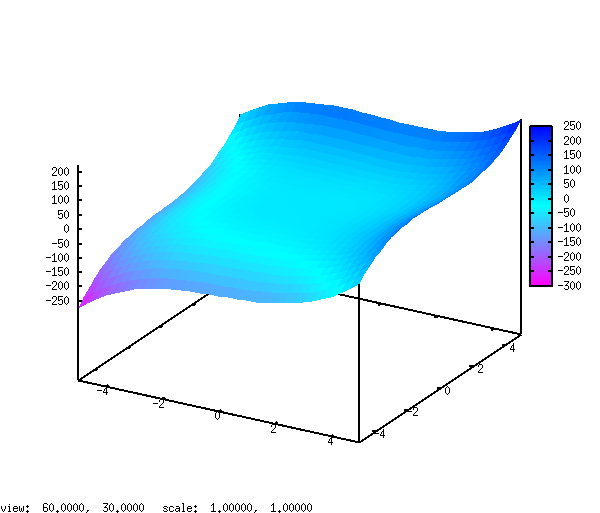
\includegraphics[scale=0.5]{7.png}
\caption{Superficie $f(x,y)= x^3+y^3+xy$ }
\end{figure}


\noindent
%%%%%%%%%%%%%%%
%%% INPUT:
\begin{minipage}[t]{8ex}{\color{red}\bf
\begin{verbatim}
(%i4) 
\end{verbatim}}
\end{minipage}
\begin{minipage}[t]{\textwidth}{\color{blue}
\begin{verbatim}
draw3d(contour_levels=10,
       contour=map,
       explicit(f(x,y),x,-5,5,y,-5,5));
\end{verbatim}}
\end{minipage}
%%% OUTPUT:
\begin{math}\displaystyle
\parbox{8ex}{\color{labelcolor}(\%o4) }
[\mathrm{gr3d}\left( explicit\right) ]
\end{math}
\begin{figure}[H]
\centering
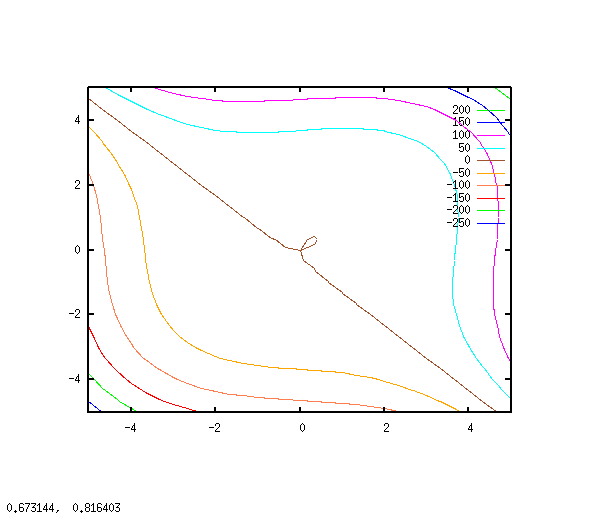
\includegraphics[scale=0.5]{8.png}
\caption{Curvas de nivel de $f(x,y)= x^3+y^3+xy$ }
\end{figure}


\noindent
%%%%%%%%%%%%%%%
%%% INPUT:
\begin{minipage}[t]{8ex}{\color{red}\bf
\begin{verbatim}
(%i5) 
\end{verbatim}}
\end{minipage}
\begin{minipage}[t]{\textwidth}{\color{blue}
\begin{verbatim}
fx : diff(f(x,y),x);
fy : diff(f(x,y),y);
solve([fx,fy],[x,y]);
\end{verbatim}}
\end{minipage}
%%% OUTPUT:
\begin{math}\displaystyle
\parbox{8ex}{\color{labelcolor}(\%o5) }
3\,{x}^{2}-y
\end{math}

\begin{math}\displaystyle
\parbox{8ex}{\color{labelcolor}(\%o6) }
3\,{y}^{2}-x
\end{math}

\begin{math}\displaystyle
\parbox{8ex}{\color{labelcolor}(\%o7) }
[[x=\frac{1}{3},y=\frac{1}{3}],[x=-\frac{\sqrt{3}\,i+1}{6},y=\frac{\sqrt{3}\,i-1}{6}],[x=\frac{\sqrt{3}\,i-1}{6},y=-\frac{\sqrt{3}\,i+1}{6}],[x=0,y=0]]
\end{math}
%%%%%%%%%%%%%%%


\noindent
%%%%%%%%%%%%%%%
%%% INPUT:
\begin{minipage}[t]{8ex}{\color{red}\bf
\begin{verbatim}
(%i8) 
\end{verbatim}}
\end{minipage}
\begin{minipage}[t]{\textwidth}{\color{blue}
\begin{verbatim}
H: hessian(f(x,y),[x,y]);
determinant(H);
\end{verbatim}}
\end{minipage}
%%% OUTPUT:
\begin{math}\displaystyle
\parbox{8ex}{\color{labelcolor}(\%o8) }
\begin{pmatrix}6\,x & -1\cr -1 & 6\,y\end{pmatrix}
\end{math}

\begin{math}\displaystyle
\parbox{8ex}{\color{labelcolor}(\%o9) }
36\,x\,y-1
\end{math}
%%%%%%%%%%%%%%%


\noindent
%%%%%%%%%%%%%%%
%%% INPUT:
\begin{minipage}[t]{8ex}{\color{red}\bf
\begin{verbatim}
(%i10) 
\end{verbatim}}
\end{minipage}
\begin{minipage}[t]{\textwidth}{\color{blue}
\begin{verbatim}
subst([x=1/3, y=1/3],diff(fx,x));
subst([x=1/3, y=1/3],determinant(H));
f(1/3,1/3);
\end{verbatim}}
\end{minipage}
%%% OUTPUT:
\begin{math}\displaystyle
\parbox{8ex}{\color{labelcolor}(\%o10) }
2
\end{math}

\begin{math}\displaystyle
\parbox{8ex}{\color{labelcolor}(\%o11) }
3
\end{math}

\begin{math}\displaystyle
\parbox{8ex}{\color{labelcolor}(\%o12) }
-\frac{1}{27}
\end{math}
%%%%%%%%%%%%%%%


\noindent
%%%%%%%%%%%%%%%
%%% INPUT:
\begin{minipage}[t]{8ex}{\color{red}\bf
\begin{verbatim}
(%i13) 
\end{verbatim}}
\end{minipage}
\begin{minipage}[t]{\textwidth}{\color{blue}
\begin{verbatim}
subst([x=0, y=0],diff(fx,x));
subst([x=0, y=0],determinant(H));
f(0,0);
\end{verbatim}}
\end{minipage}
%%% OUTPUT:
\begin{math}\displaystyle
\parbox{8ex}{\color{labelcolor}(\%o13) }
0
\end{math}

\begin{math}\displaystyle
\parbox{8ex}{\color{labelcolor}(\%o14) }
-1
\end{math}

\begin{math}\displaystyle
\parbox{8ex}{\color{labelcolor}(\%o15) }
0
\end{math}

%===========================================================

\subsection{Multiplicadores de Lagrange}
\noindent
%%%%%%%%%%%%%%%
%%% INPUT:
\begin{minipage}[t]{8ex}{\color{red}\bf
\begin{verbatim}
(%i1) 
\end{verbatim}}
\end{minipage}
\begin{minipage}[t]{\textwidth}{\color{blue}
\begin{verbatim}
f(x,y) := x^2+2*y^2;
g : y^2+x^2;
\end{verbatim}}
\end{minipage}
%%% OUTPUT:
\begin{math}\displaystyle
\parbox{8ex}{\color{labelcolor}(\%o1) }
\mathrm{f}\left( x,y\right) :={x}^{2}+2\,{y}^{2}
\end{math}

\begin{math}\displaystyle
\parbox{8ex}{\color{labelcolor}(\%o2) }
{y}^{2}+{x}^{2}
\end{math}
%%%%%%%%%%%%%%%


\noindent
%%%%%%%%%%%%%%%
%%% INPUT:
\begin{minipage}[t]{8ex}{\color{red}\bf
\begin{verbatim}
(%i3) 
\end{verbatim}}
\end{minipage}
\begin{minipage}[t]{\textwidth}{\color{blue}
\begin{verbatim}
eq1: diff(f(x,y),x)=h*diff(g,x);
eq2: diff(f(x,y),y)=h*diff(g,y);
eq3: g=1;
\end{verbatim}}
\end{minipage}
%%% OUTPUT:
\begin{math}\displaystyle
\parbox{8ex}{\color{labelcolor}(\%o3) }
2\,x=2\,h\,x
\end{math}

\begin{math}\displaystyle
\parbox{8ex}{\color{labelcolor}(\%o4) }
4\,y=2\,h\,y
\end{math}

\begin{math}\displaystyle
\parbox{8ex}{\color{labelcolor}(\%o5) }
{y}^{2}+{x}^{2}=1
\end{math}
%%%%%%%%%%%%%%%


\noindent
%%%%%%%%%%%%%%%
%%% INPUT:
\begin{minipage}[t]{8ex}{\color{red}\bf
\begin{verbatim}
(%i6) 
\end{verbatim}}
\end{minipage}
\begin{minipage}[t]{\textwidth}{\color{blue}
\begin{verbatim}
solve([eq1,eq2,eq3],[x,y,h]);
\end{verbatim}}
\end{minipage}
%%% OUTPUT:
\begin{math}\displaystyle
\parbox{8ex}{\color{labelcolor}(\%o6) }
[[x=1,y=0,h=1],[x=-1,y=0,h=1],[x=0,y=-1,h=2],[x=0,y=1,h=2]]
\end{math}
%%%%%%%%%%%%%%%


\noindent
%%%%%%%%%%%%%%%
%%% INPUT:
\begin{minipage}[t]{8ex}{\color{red}\bf
\begin{verbatim}
(%i7) 
\end{verbatim}}
\end{minipage}
\begin{minipage}[t]{\textwidth}{\color{blue}
\begin{verbatim}
[f(1,0),f(-1,0),f(0,-1),f(0,1)];
\end{verbatim}}
\end{minipage}
%%% OUTPUT:
\begin{math}\displaystyle
\parbox{8ex}{\color{labelcolor}(\%o7) }
[1,1,2,2]
\end{math}

%===========================================================

\section{Integración Multiple}
Maxima nos permite realizar integrales de varias variables.
\subsection{Integrales Dobles}
Con el comando \texttt{integrate()} nos permite realizar las integrales . 

\noindent
%%%%%%%%%%%%%%%
%%% INPUT:
\begin{minipage}[t]{8ex}{\color{red}\bf
\begin{verbatim}
(%i1) 
\end{verbatim}}
\end{minipage}
\begin{minipage}[t]{\textwidth}{\color{blue}
\begin{verbatim}
f: 4*x^3-4*x*y;
\end{verbatim}}
\end{minipage}
%%% OUTPUT:
\begin{math}\displaystyle
\parbox{8ex}{\color{labelcolor}(\%o1) }
4\,{x}^{3}-4\,x\,y
\end{math}
%%%%%%%%%%%%%%%


\noindent
%%%%%%%%%%%%%%%
%%% INPUT:
\begin{minipage}[t]{8ex}{\color{red}\bf
\begin{verbatim}
(%i2) 
\end{verbatim}}
\end{minipage}
\begin{minipage}[t]{\textwidth}{\color{blue}
\begin{verbatim}
integrate(integrate(f,y),x);
\end{verbatim}}
\end{minipage}
%%% OUTPUT:
\begin{math}\displaystyle
\parbox{8ex}{\color{labelcolor}(\%o2) }
{x}^{4}\,y-{x}^{2}\,{y}^{2}
\end{math}
%%%%%%%%%%%%%%%


\noindent
%%%%%%%%%%%%%%%
%%% INPUT:
\begin{minipage}[t]{8ex}{\color{red}\bf
\begin{verbatim}
(%i3) 
\end{verbatim}}
\end{minipage}
\begin{minipage}[t]{\textwidth}{\color{blue}
\begin{verbatim}
integrate(integrate(f,y,x^1/2,2-x),x,0,1);
\end{verbatim}}
\end{minipage}
%%% OUTPUT:
\begin{math}\displaystyle
\parbox{8ex}{\color{labelcolor}(\%o3) }
-\frac{109}{120}
\end{math}
%============================================================

\subsection{Coordenadas Polares}
Con maxima se puede cambiar a coordenadas polares para facilitar el calculo.

\noindent
%%%%%%%%%%%%%%%
%%% INPUT:
\begin{minipage}[t]{8ex}{\color{red}\bf
\begin{verbatim}
(%i1) 
\end{verbatim}}
\end{minipage}
\begin{minipage}[t]{\textwidth}{\color{blue}
\begin{verbatim}
f(x,y):= 4*x^2+4*y^2;
\end{verbatim}}
\end{minipage}
%%% OUTPUT:
\begin{math}\displaystyle
\parbox{8ex}{\color{labelcolor}(\%o1) }
\mathrm{f}\left( x,y\right) :=4\,{x}^{2}+4\,{y}^{2}
\end{math}
%%%%%%%%%%%%%%%


\noindent
%%%%%%%%%%%%%%%
%%% INPUT:
\begin{minipage}[t]{8ex}{\color{red}\bf
\begin{verbatim}
(%i2) 
\end{verbatim}}
\end{minipage}
\begin{minipage}[t]{\textwidth}{\color{blue}
\begin{verbatim}
[x,y]: [r*cos(theta), r*sin(theta)];
\end{verbatim}}
\end{minipage}
%%% OUTPUT:
\begin{math}\displaystyle
\parbox{8ex}{\color{labelcolor}(\%o2) }
[r\,\mathrm{cos}\left( \theta\right) ,r\,\mathrm{sin}\left( \theta\right) ]
\end{math}
%%%%%%%%%%%%%%%


\noindent
%%%%%%%%%%%%%%%
%%% INPUT:
\begin{minipage}[t]{8ex}{\color{red}\bf
\begin{verbatim}
(%i3) 
\end{verbatim}}
\end{minipage}
\begin{minipage}[t]{\textwidth}{\color{blue}
\begin{verbatim}
integrate(integrate(f(x,y)*r,r,0,2*cos(theta)),theta,-%pi/2,%pi/2);
\end{verbatim}}
\end{minipage}
%%% OUTPUT:
\begin{math}\displaystyle
\parbox{8ex}{\color{labelcolor}(\%o3) }
6\,\pi 
\end{math}
%===========================================================

\subsection{Integrales Triples}
Tambien es posible realizar integrales de 3 parametros.

\noindent
%%%%%%%%%%%%%%%
%%% INPUT:
\begin{minipage}[t]{8ex}{\color{red}\bf
\begin{verbatim}
(%i1) 
\end{verbatim}}
\end{minipage}
\begin{minipage}[t]{\textwidth}{\color{blue}
\begin{verbatim}
f(x,y,z):= x^2*y*z;
integrate(integrate(integrate(f(x,y,z),z,0,x+y),y,0,-x),x,0,1);
\end{verbatim}}
\end{minipage}
%%% OUTPUT:
\begin{math}\displaystyle
\parbox{8ex}{\color{labelcolor}(\%o1) }
\mathrm{f}\left( x,y,z\right) :={x}^{2}\,y\,z
\end{math}

\begin{math}\displaystyle
\parbox{8ex}{\color{labelcolor}(\%o2) }
\frac{1}{168}
\end{math}
%==================================================

\subsection{Integreles en Coordenadas Cilindricas y Esfericas}
Con maxima se puede cambiar a otras coordenadas para facilitar el calculo.

\noindent
%%%%%%%%%%%%%%%
%%% INPUT:
\begin{minipage}[t]{8ex}{\color{red}\bf
\begin{verbatim}
(%i1) 
\end{verbatim}}
\end{minipage}
\begin{minipage}[t]{\textwidth}{\color{blue}
\begin{verbatim}
f(x,y,z):= y*z;
[x,y,z]:[r*cos(theta),r*sin(theta),z];
integrate(integrate(integrate(f(x,y,z)*r,z,0,3),r,0,2),theta,0,%pi);
kill(f,x,y,z);
\end{verbatim}}
\end{minipage}
%%% OUTPUT:
\begin{math}\displaystyle
\parbox{8ex}{\color{labelcolor}(\%o1) }
\mathrm{f}\left( x,y,z\right) :=y\,z
\end{math}

\begin{math}\displaystyle
\parbox{8ex}{\color{labelcolor}(\%o2) }
[r\,\mathrm{cos}\left( \theta\right) ,r\,\mathrm{sin}\left( \theta\right) ,z]
\end{math}

\begin{math}\displaystyle
\parbox{8ex}{\color{labelcolor}(\%o3) }
24
\end{math}

\begin{math}\displaystyle
\parbox{8ex}{\color{labelcolor}(\%o4) }
done
\end{math}
%%%%%%%%%%%%%%%


\noindent
%%%%%%%%%%%%%%%
%%% INPUT:
\begin{minipage}[t]{8ex}{\color{red}\bf
\begin{verbatim}
(%i5) 
\end{verbatim}}
\end{minipage}
\begin{minipage}[t]{\textwidth}{\color{blue}
\begin{verbatim}
f(x,y,z):= x*z;
[x,y,z]: [rho*sin(phi)*cos(theta),rho*sin(phi)*sin(theta),rho*cos(phi)];
integrate(integrate(integrate(f(x,y,z)*rho^2*sin(phi),rho,0,1),theta,0,%pi),phi,0,%pi/2);
kill(f,x,y,z);
\end{verbatim}}
\end{minipage}
%%% OUTPUT:
\begin{math}\displaystyle
\parbox{8ex}{\color{labelcolor}(\%o5) }
\mathrm{f}\left( x,y,z\right) :=x\,z
\end{math}

\begin{math}\displaystyle
\parbox{8ex}{\color{labelcolor}(\%o6) }
[\mathrm{sin}\left( \phi\right) \,\rho\,\mathrm{cos}\left( \theta\right) ,\mathrm{sin}\left( \phi\right) \,\rho\,\mathrm{sin}\left( \theta\right) ,\mathrm{cos}\left( \phi\right) \,\rho]
\end{math}

\begin{math}\displaystyle
\parbox{8ex}{\color{labelcolor}(\%o7) }
0
\end{math}

\begin{math}\displaystyle
\parbox{8ex}{\color{labelcolor}(\%o8) }
done
\end{math}
%============================================================0

\subsection{Cambio de variable}
Con maxima se puede realizar cambio variable para facilitar el calculo.

\noindent
%%%%%%%%%%%%%%%
%%% INPUT:
\begin{minipage}[t]{8ex}{\color{red}\bf
\begin{verbatim}
(%i1) 
\end{verbatim}}
\end{minipage}
\begin{minipage}[t]{\textwidth}{\color{blue}
\begin{verbatim}
f(x,y) := x+y;
[x,y]: [u^3-v^4, 5*u*v];
\end{verbatim}}
\end{minipage}
%%% OUTPUT:
\begin{math}\displaystyle
\parbox{8ex}{\color{labelcolor}(\%o1) }
\mathrm{f}\left( x,y\right) :=x+y
\end{math}

\begin{math}\displaystyle
\parbox{8ex}{\color{labelcolor}(\%o2) }
[{u}^{3}-{v}^{4},5\,u\,v]
\end{math}
%%%%%%%%%%%%%%%


\noindent
%%%%%%%%%%%%%%%
%%% INPUT:
\begin{minipage}[t]{8ex}{\color{red}\bf
\begin{verbatim}
(%i3) 
\end{verbatim}}
\end{minipage}
\begin{minipage}[t]{\textwidth}{\color{blue}
\begin{verbatim}
J: jacobian([x,y],[u,v]);
J: determinant(J);
\end{verbatim}}
\end{minipage}
%%% OUTPUT:
\begin{math}\displaystyle
\parbox{8ex}{\color{labelcolor}(\%o3) }
\begin{pmatrix}3\,{u}^{2} & -4\,{v}^{3}\cr 5\,v & 5\,u\end{pmatrix}
\end{math}

\begin{math}\displaystyle
\parbox{8ex}{\color{labelcolor}(\%o4) }
20\,{v}^{4}+15\,{u}^{3}
\end{math}
%%%%%%%%%%%%%%%


\noindent
%%%%%%%%%%%%%%%
%%% INPUT:
\begin{minipage}[t]{8ex}{\color{red}\bf
\begin{verbatim}
(%i5) 
\end{verbatim}}
\end{minipage}
\begin{minipage}[t]{\textwidth}{\color{blue}
\begin{verbatim}
integrate(integrate(f(x,y)*J,u,1,2),v,3,4);
\end{verbatim}}
\end{minipage}
%%% OUTPUT:
\begin{math}\displaystyle
\parbox{8ex}{\color{labelcolor}(\%o5) }
-\frac{113349305}{252}
\end{math}
%==========================================================

\section{Cálculo Vectorial}
Maxima nos permite trabajar con campos vectoriales.
\subsection{Campo Vectorial}
Maxima nos permite graficar los campos vectoriales

\noindent
%%%%%%%%%%%%%%%
%%% INPUT:
\begin{minipage}[t]{8ex}{\color{red}\bf
\begin{verbatim}
(%i1) 
\end{verbatim}}
\end{minipage}
\begin{minipage}[t]{\textwidth}{\color{blue}
\begin{verbatim}
load(draw);
load(vect);
F(x,y):= (x^2,y^2);
\end{verbatim}}
\end{minipage}
%%% OUTPUT:
\begin{math}\displaystyle
\parbox{8ex}{\color{labelcolor}(\%o1) }
/usr/share/maxima/5.34.1/share/draw/draw.lisp
\end{math}

\begin{math}\displaystyle
\parbox{8ex}{\color{labelcolor}(\%o2) }
/usr/share/maxima/5.34.1/share/vector/vect.mac
\end{math}

\begin{math}\displaystyle
\parbox{8ex}{\color{labelcolor}(\%o3) }
\mathrm{F}\left( x,y\right) :=\left( {x}^{2},{y}^{2}\right) 
\end{math}
%%%%%%%%%%%%%%%


\subparagraph{Campo Vectorial Dos Dimensiones:}
Graficación del campo vectorial.

\noindent
%%%%%%%%%%%%%%%
%%% INPUT:
\begin{minipage}[t]{8ex}{\color{red}\bf
\begin{verbatim}
(%i4) 
\end{verbatim}}
\end{minipage}
\begin{minipage}[t]{\textwidth}{\color{blue}
\begin{verbatim}
coord: setify(makelist(k,k,-6,6));
points2d :listify(cartesian_product(coord,coord));
vf2d(x,y):= vector([x,y],[4*cos(y),x^2]/10);
vect2: makelist(vf2d(k[1],k[2]), k, points2d);
apply ( draw2d , append ([head_length=0.2], [color = green ] , vect2 ));
\end{verbatim}}
\end{minipage}

\begin{figure}[H]
\centering
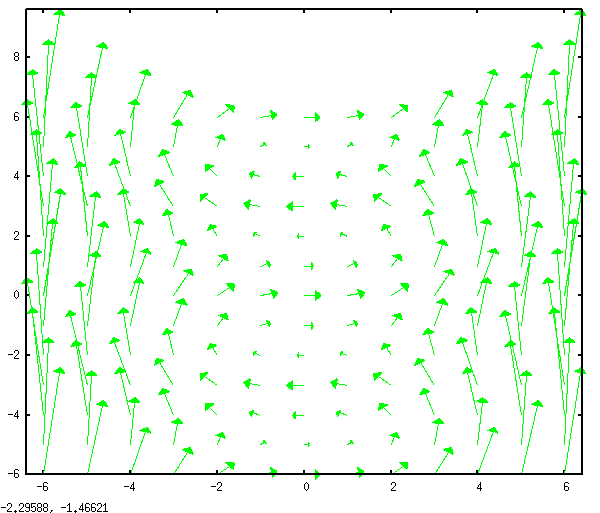
\includegraphics[scale=0.5]{9.png}
\caption{Campo  $f(x,y)= (4\cos(y),x^2)$ }
\end{figure}


\subparagraph{Campo Gradiente:}
Graficación del Campo Gradiente.

\noindent
%%%%%%%%%%%%%%%
%%% INPUT:
\begin{minipage}[t]{8ex}{\color{red}\bf
\begin{verbatim}
(%i9) 
\end{verbatim}}
\end{minipage}
\begin{minipage}[t]{\textwidth}{\color{blue}
\begin{verbatim}
kill(f,x,y,gdf);
f(x,y) := cos(x^2) - y^2;
scalefactors ([ x , y ]);
gdf(x,y):= grad(f(x,y));
ev(express(gdf(x,y)),diff);
define(gdf(x,y),%);
\end{verbatim}}
\end{minipage}

\noindent
%%%%%%%%%%%%%%%
%%% INPUT:
\begin{minipage}[t]{8ex}{\color{red}\bf
\begin{verbatim}
(%i15) 
\end{verbatim}}
\end{minipage}
\begin{minipage}[t]{\textwidth}{\color{blue}
\begin{verbatim}
coord: setify(makelist(k,k,-6,6));
points2d : listify(cartesian_product(coord,coord));
vf2d(x,y):= vector([x,y],gdf(x,y)/10);
vect2: makelist(vf2d(k[1],k[2]),k, points2d);
apply(draw2d, append([head_length=0.25, color=green], vect2));
\end{verbatim}}
\end{minipage}

\begin{figure}[H]
\centering
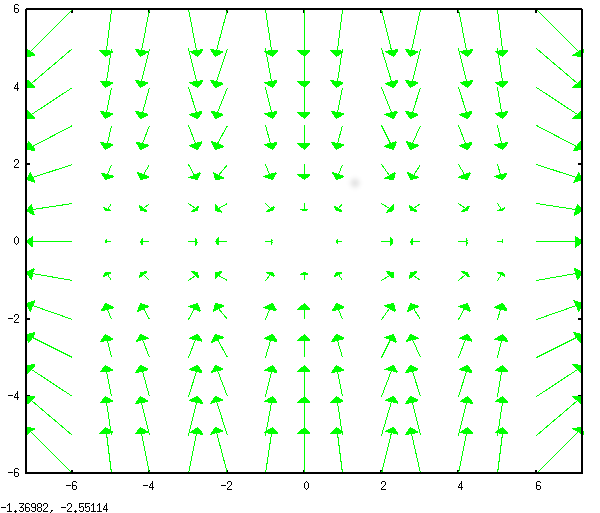
\includegraphics[scale=0.5]{10.png}
\caption{Campo gradiente  $f(x,y)= (-2x\sin(x^2),-2y)$ }
\end{figure}


\subparagraph{Campo Vectorial Tres Dimensiones:}
Graficación Campo vectorial 3 dimensiones.

\noindent
%%%%%%%%%%%%%%%
%%% INPUT:
\begin{minipage}[t]{8ex}{\color{red}\bf
\begin{verbatim}
(%i20) 
\end{verbatim}}
\end{minipage}
\begin{minipage}[t]{\textwidth}{\color{blue}
\begin{verbatim}
coord: setify(makelist(k,k,-3,3));
points3d : listify(cartesian_product(coord, coord, coord));
vf3d(x,y,z):= vector([x,y,z],[z,x*z,y]/8);
vect3 : makelist(vf3d(k[1],k[2],k[3]),k,points3d);
apply(draw3d, append([color=red,head_length=0.1],vect3));
\end{verbatim}}
\end{minipage}

\begin{figure}[H]
\centering
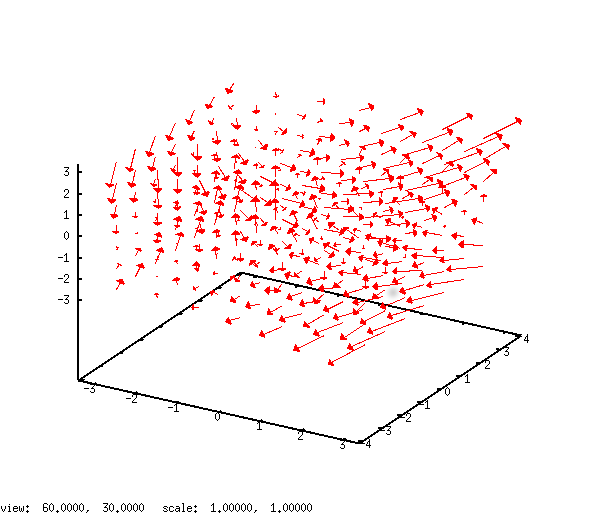
\includegraphics[scale=0.65]{11.png}
\caption{Campo $f(x,y,z)= (z,xz,y)$ }
\end{figure}
 %============================================================
 
\subsection{Integral de Linea}
Con maxima es simple realizar una integral de linea.

\noindent
%%%%%%%%%%%%%%%
%%% INPUT:
\begin{minipage}[t]{8ex}{\color{red}\bf
\begin{verbatim}
(%i1) 
\end{verbatim}}
\end{minipage}
\begin{minipage}[t]{\textwidth}{\color{blue}
\begin{verbatim}
f(x,y) := x^2+y^2;
[x,y] : [cos(t), sin(2*t)];
rp: diff([x,y],t);
romberg(f(x,y)*sqrt(rp.rp), t, 0,1);
\end{verbatim}}
\end{minipage}
%%% OUTPUT:
\begin{math}\displaystyle
\parbox{8ex}{\color{labelcolor}(\%o1) }
\mathrm{f}\left( x,y\right) :={x}^{2}+{y}^{2}
\end{math}

\begin{math}\displaystyle
\parbox{8ex}{\color{labelcolor}(\%o2) }
[\mathrm{cos}\left( t\right) ,\mathrm{sin}\left( 2\,t\right) ]
\end{math}

\begin{math}\displaystyle
\parbox{8ex}{\color{labelcolor}(\%o3) }
[-\mathrm{sin}\left( t\right) ,2\,\mathrm{cos}\left( 2\,t\right) ]
\end{math}

\begin{math}\displaystyle
\parbox{8ex}{\color{labelcolor}(\%o4) }
1.635879048260742
\end{math}
%%%%%%%%%%%%%%%


\noindent
%%%%%%%%%%%%%%%
%%% INPUT:
\begin{minipage}[t]{8ex}{\color{red}\bf
\begin{verbatim}
(%i5) 
\end{verbatim}}
\end{minipage}
\begin{minipage}[t]{\textwidth}{\color{blue}
\begin{verbatim}
F(x,y,z) := [-x*y^3, x*z, y*z^2];
[x,y,z]: [t^2,t^3,t^4];
romberg(F(x,y,z).diff([x,y,z],t),t,0,1);
\end{verbatim}}
\end{minipage}
%%% OUTPUT:
\begin{math}\displaystyle
\parbox{8ex}{\color{labelcolor}(\%o5) }
\mathrm{F}\left( x,y,z\right) :=[\left( -x\right) \,{y}^{3},x\,z,y\,{z}^{2}]
\end{math}

\begin{math}\displaystyle
\parbox{8ex}{\color{labelcolor}(\%o6) }
[{t}^{2},{t}^{3},{t}^{4}]
\end{math}

\begin{math}\displaystyle
\parbox{8ex}{\color{labelcolor}(\%o7) }
0.4461538461603604
\end{math}

%====================================================
\subsection{Campos Conservativos y Encontrando Potenciales Escalares}
Con la función \texttt{curl()} podemos ver si los campos son conservativos, y  podemos encontrar el potencial escalar con la función \texttt{potential()}.
 
 \noindent
%%%%%%%%%%%%%%%
%%% INPUT:
\begin{minipage}[t]{8ex}{\color{red}\bf
\begin{verbatim}
(%i1) 
\end{verbatim}}
\end{minipage}
\begin{minipage}[t]{\textwidth}{\color{blue}
\begin{verbatim}
load(vect);
F(x,y):= [4*x^3-5*y^2,5*y^3-3*x];
scalefactors([x,y]);
\end{verbatim}}
\end{minipage}
%%% OUTPUT:
\begin{math}\displaystyle
\parbox{8ex}{\color{labelcolor}(\%o1) }
/usr/share/maxima/5.34.1/share/vector/vect.mac
\end{math}

\begin{math}\displaystyle
\parbox{8ex}{\color{labelcolor}(\%o2) }
\mathrm{F}\left( x,y\right) :=[4\,{x}^{3}-5\,{y}^{2},5\,{y}^{3}-3\,x]
\end{math}

\begin{math}\displaystyle
\parbox{8ex}{\color{labelcolor}(\%o3) }
done
\end{math}
%%%%%%%%%%%%%%%


\noindent
%%%%%%%%%%%%%%%
%%% INPUT:
\begin{minipage}[t]{8ex}{\color{red}\bf
\begin{verbatim}
(%i4) 
\end{verbatim}}
\end{minipage}
\begin{minipage}[t]{\textwidth}{\color{blue}
\begin{verbatim}
curl(F(x,y));
express(%);
ev(%,diff);
\end{verbatim}}
\end{minipage}
%%% OUTPUT:
\begin{math}\displaystyle
\parbox{8ex}{\color{labelcolor}(\%o4) }
\mathrm{curl}\left( [4\,{x}^{3}-5\,{y}^{2},5\,{y}^{3}-3\,x]\right) 
\end{math}

\begin{math}\displaystyle
\parbox{8ex}{\color{labelcolor}(\%o5) }
\frac{d}{d\,x}\,\left( 5\,{y}^{3}-3\,x\right) -\frac{d}{d\,y}\,\left( 4\,{x}^{3}-5\,{y}^{2}\right) 
\end{math}

\begin{math}\displaystyle
\parbox{8ex}{\color{labelcolor}(\%o6) }
10\,y-3
\end{math}
%%%%%%%%%%%%%%%


\noindent
%%%%%%%%%%%%%%%
%%% INPUT:
\begin{minipage}[t]{8ex}{\color{red}\bf
\begin{verbatim}
(%i7) 
\end{verbatim}}
\end{minipage}
\begin{minipage}[t]{\textwidth}{\color{blue}
\begin{verbatim}
F(x,y):= [x^3+5*y,5*y^3+5*x];
ev(express(curl(F(x,y))),diff);
\end{verbatim}}
\end{minipage}
%%% OUTPUT:
\begin{math}\displaystyle
\parbox{8ex}{\color{labelcolor}(\%o7) }
\mathrm{F}\left( x,y\right) :=[{x}^{3}+5\,y,5\,{y}^{3}+5\,x]
\end{math}

\begin{math}\displaystyle
\parbox{8ex}{\color{labelcolor}(\%o8) }
0
\end{math}
%%%%%%%%%%%%%%%


\noindent
%%%%%%%%%%%%%%%
%%% INPUT:
\begin{minipage}[t]{8ex}{\color{red}\bf
\begin{verbatim}
(%i9) 
\end{verbatim}}
\end{minipage}
\begin{minipage}[t]{\textwidth}{\color{blue}
\begin{verbatim}
F(u,v):= [u^3+5*v,5*v^3+5*u];
scalefactors([u,v]);
potential(F(u,v));
define(f(u,v),%);
f(2,3)-f(0,1);
\end{verbatim}}
\end{minipage}
%%% OUTPUT:
\begin{math}\displaystyle
\parbox{8ex}{\color{labelcolor}(\%o9) }
\mathrm{F}\left( u,v\right) :=[{u}^{3}+5\,v,5\,{v}^{3}+5\,u]
\end{math}

\begin{math}\displaystyle
\parbox{8ex}{\color{labelcolor}(\%o10) }
done
\end{math}

\begin{math}\displaystyle
\parbox{8ex}{\color{labelcolor}(\%o11) }
\frac{5\,{v}^{4}+20\,u\,v+{u}^{4}}{4}
\end{math}

\begin{math}\displaystyle
\parbox{8ex}{\color{labelcolor}(\%o12) }
\mathrm{f}\left( u,v\right) :=\frac{5\,{v}^{4}+20\,u\,v+{u}^{4}}{4}
\end{math}

\begin{math}\displaystyle
\parbox{8ex}{\color{labelcolor}(\%o13) }
134
\end{math}

\begin{thebibliography}{3}
\bibitem{M}
Source Forge,
\emph{Maxima}. Recuperado en abril de 2016 de \url{http://maxima.sourceforge.net/es/}

\bibitem{JK}
Kerns, Jay.
\emph{Multivariable Calculus with Maxima}. Recuperado en abril de 2016 de \url{http://gkerns.people.ysu.edu/maxima/maximaintro/}

\bibitem{FC}
Lizárraga, C.
\emph{Actividad 8 (2016-1)}. Recuperado en abril de 2016 de \url{http://computacional1.pbworks.com/w/page/106192917/Actividad\%208\%20(2016-1)}
\end{thebibliography}



\end{document}

